\pdfbookmark[1]{Super_conducting_qubits}{Super_conducting_qubits}
\chapter{Superconducting qubits}\label{chap:Super_conducting_qubits}



\section{Interaction of atoms and electromagnetic waves}
    In superconducting circuits, it is the ?? find out elements of the Josephson junction which constitute our qubits in our \acrshort{qpu} and the electromagnetic waves we use to control and manipulate the qubits. For this it is important to know what happens when they interact. Therefore, we will dig deeper into how we can describe the interaction between electromagnetic waves and the 2 level qubits using the Jaynes cummings hamiltonian. Typically the qubits are operated within the microwave-range corresponding to frequencies 
    \\
    Write what you find out in quantum optics course. 
        laser (coherent state?) interacting with a 2 level system in a cavity? is it really a cavity? ask peter. 
    \\
    A series of specific manipulations (rotations) are called gates. 
    \\
    Talk about how we use light to go around on the bloch sphere. 
    \\
    In quantum computing we want some very specific ways of manipulating out qubits (gates) which are discussed in the next section.
    
        
\section{Superconducting circuits architecture}
    A classical circuit consists of components like capacitors, inductors, and resistors. The components are referred to as branches and these are connected by wires called nodes \cite{Griffiths2018}. A closed path where each node and branch only are represented once, is called a loop. One can utilize superconducting materials in order to fabricate the circuit components. Doing so, quantum mechanic effects will be non-neglectful and should be taken into account \cite{Girvin2014}. The strategy for describing the dynamics in quantum circuits is to use analytical mechanics and electrodynamics. Then we will quantize the charge and the flux to end up with the Hamiltonian of our system \cite{Krantz2019}. We relate the magnetic flux to the phase as  $\Phi= \frac{1}{2\pi}\Phi_{0} \phi \Rightarrow \phi = \frac{\Phi 2 \pi}{\Phi_0}$. The phase can also be interpreted as the reduced flux quantum. The fundamental building blocks of a quantum computer is the above mentioned compnents. (Mention also the capacitor) the JJ junction, the resonator and the Josephson junction array which work as an inductor. You can put them together in many different ways in order to obtain the right properties.  Then the energies of the different components are: 
    \begin{equation}
        \begin{aligned}
            Capacitor:& \quad h_C  = \frac{C}{2} \Dot{\Phi}^2     \\ 
            Inductor:& \quad h_L = \frac{1}{2 L} \Phi^2    \\
            Josephson:& \quad h_{J} = E_j \cos \left(\frac{\Phi 2 \pi}{\Phi_0} \right)    \\
        \end{aligned}
    \end{equation}
    Where $\Phi_{0}=\frac{h}{2e}$ is the flux quantum and $\Phi$ is our conjugated position. Since the Lagrangian depend on $\Phi$ and $\Dot{\Phi}$, We obtain the conjugated momentum:
    \begin{equation}
        q = \frac{\partial \mathcal{L}}{\partial \dot{\Phi}} = \frac{2 e}{\hbar} \frac{\partial \mathcal{L}}{\partial \dot{\phi}}
    \end{equation}
    Then the Hamiltonian of our system can by found by doing a Legendre transformation.
    \begin{equation}
        \mathcal{H}  =\dot{\Phi} q-\mathcal{L}=\frac{\hbar}{2 e} \dot{\phi} q-\mathcal{L}
    \end{equation}
    Now that we have defined the conjugated variables, we can calculate the Poisson bracket
    \\
    We have that the commutation relation between our quantized  variables, $\hat{q}$ and $\hat{\Phi}$ to obtain \cite{Girvin2014}:
    \begin{equation}
        [\hat{\Phi}, \hat{q}] = \hat{\Phi} \hat{q} -\hat{q} \hat{\Phi} = i \hbar
    \end{equation}
    Therefore, $\hat{\Phi}$ and $\hat{q}$ is analogous to the position and the momentum. Further, we can define the reduced charge as \cite{Girvin2014}: 
    \begin{equation}
        \hat{n} = \frac{\hat{q}}{2e}
    \end{equation}
    Where $\hat{n}$ is an operator which gives the number of cooper pairs in a state. From now on, we skip the hat on any operator. From this, we can find the eigen energies and eigen states of the system. The energy difference between 2 levels, lets say the 0th and 1st level, are given by $\hbar \omega_{01} = E_1 - E_2 $. We can further define the anharmonicity, a, to be the change in energy difference. The anharmonicity between $\hbar\omega_{01}$ and $\hbar\omega_{21}$ = $a = \hbar\omega_{10}-\hbar\omega_{21}$. 
    \newline
    \newline
    In order to build a quantum computer, DiVincenzo's criteria should be fulfilled \cite{DiVincenzo2000}. DiVincenzo's criteria are a set of five requirements for a practical quantum computer, including qubit Initialization, strong qubit control, long coherence times, scalability, and fast measurement. Since the classical \acrshort{cpu} is made of electronic circuits, the superconducting circuits are a natural choice for implementing a \acrshort{qpu} (qubits). In this project, the focus is at the properties of the qubit. The qubit should be a well defined and stable 2 level system. This is achieved by engineering the energy spectrum of the superconducting circuit, that is the energy spectrum of the cooper pairs, so that the 2 lowest lying energy levels is well defined with a large anharmonicity to the following states.
\section{The Transmon}
    \begin{figure}
        \centering
        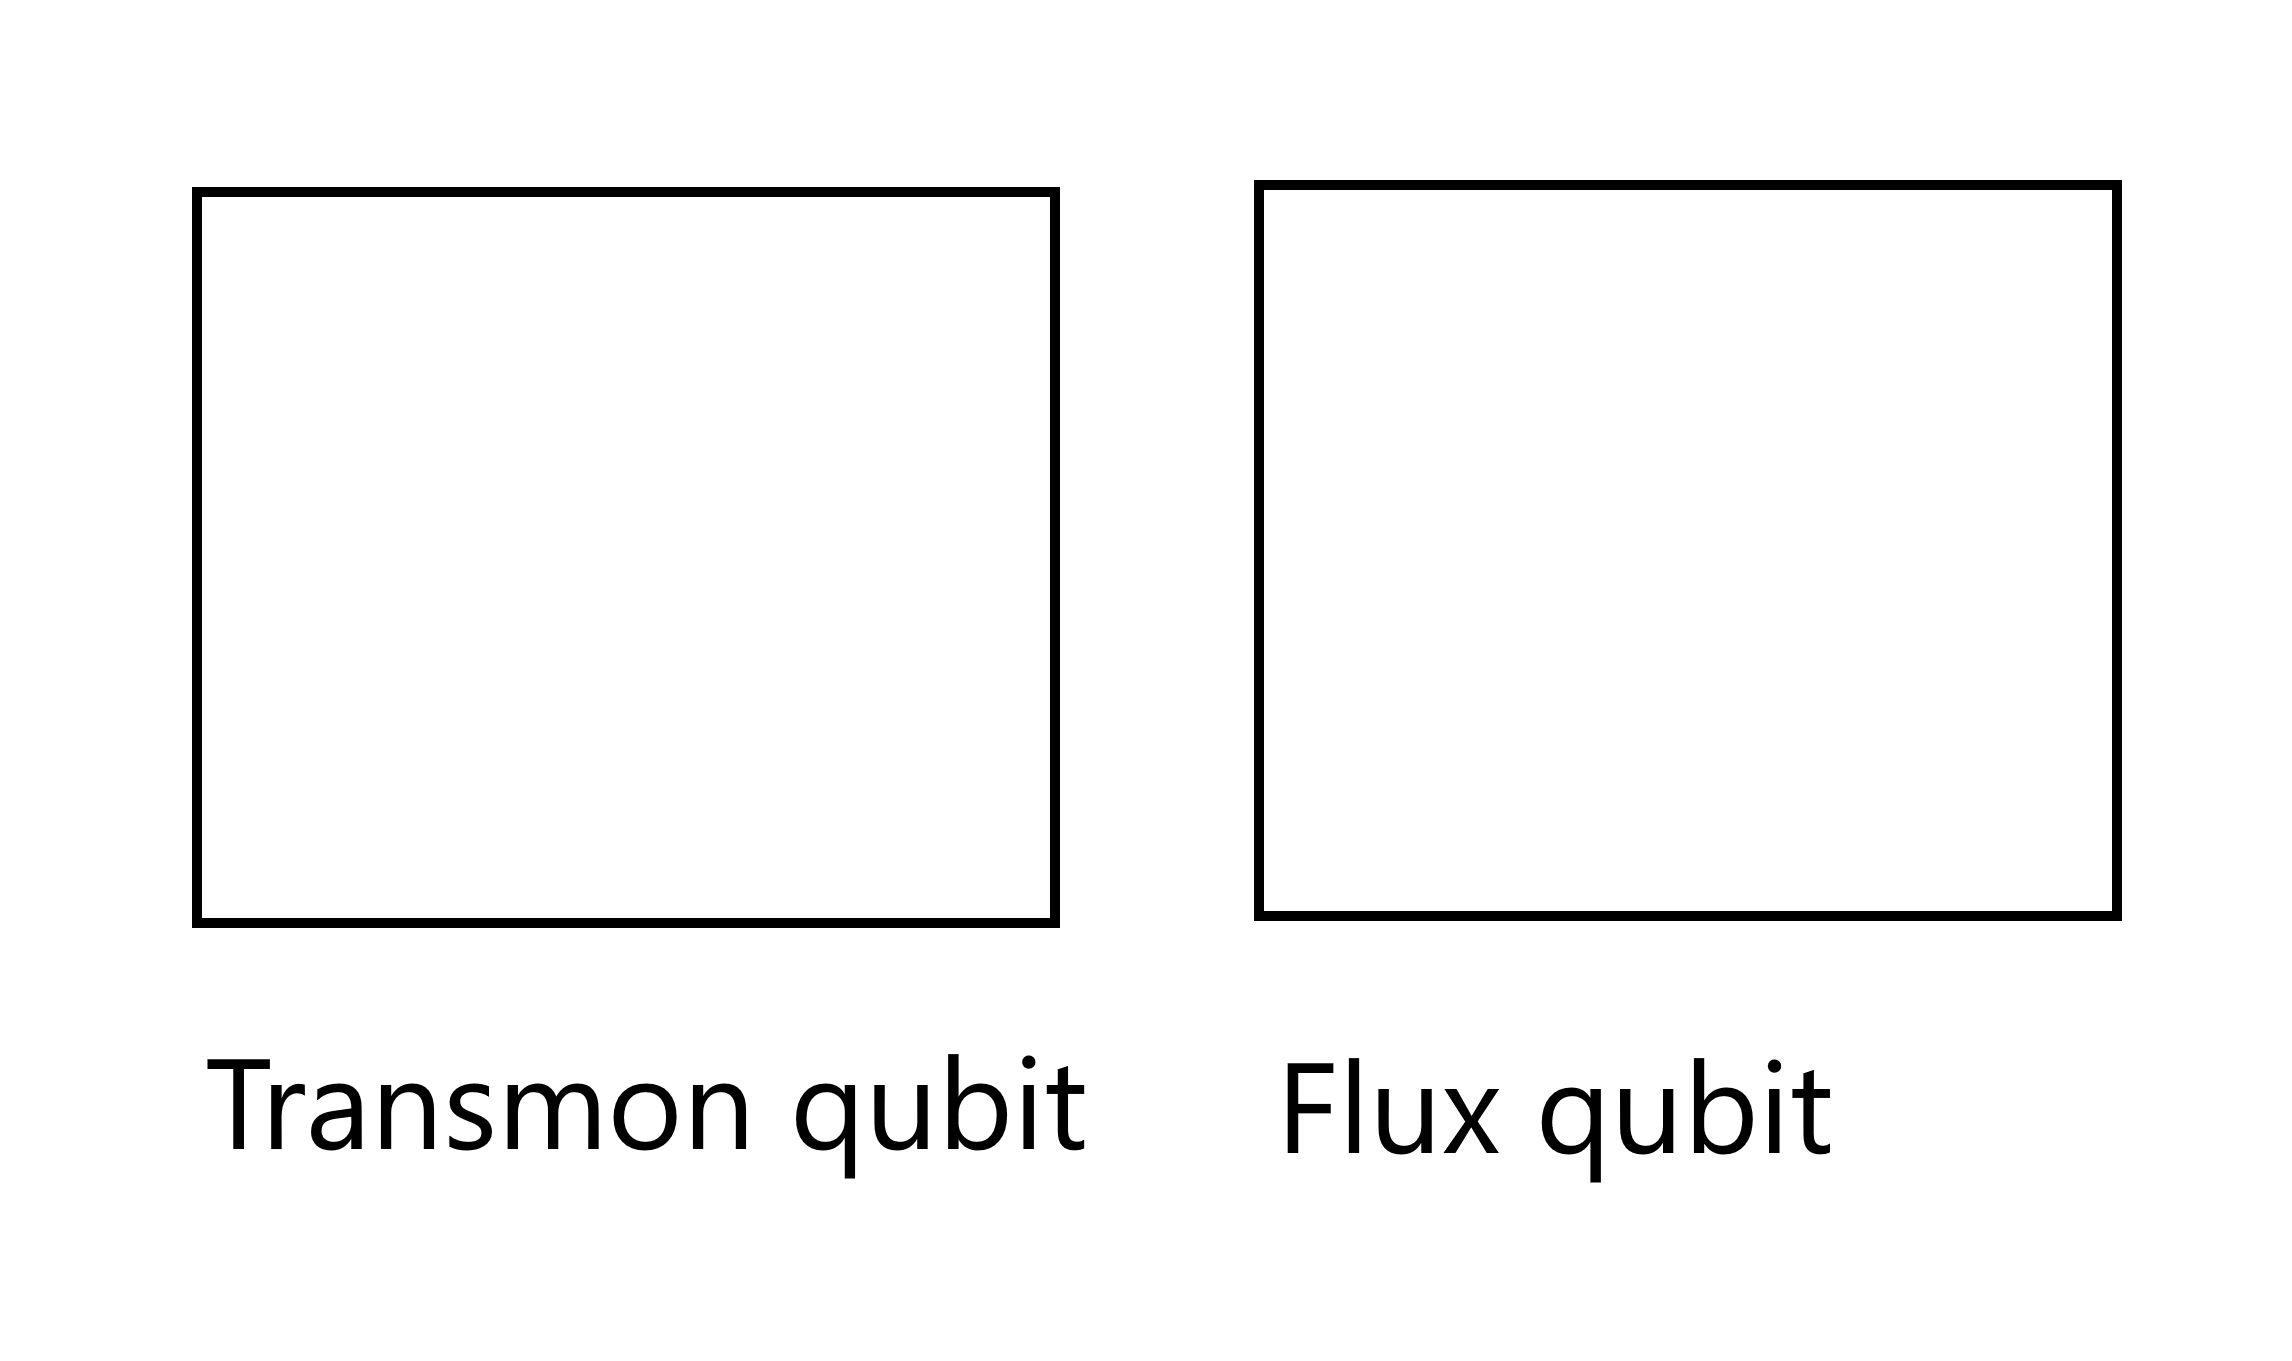
\includegraphics[width = 13 cm]{Images/Transmon and flux-qubit.png}
        \caption[Circuit diagram of Transmon and Flux qubits]{\textbf{Circuit diagram of Transmon and Flux qubits:} Model of the Transmon qubit (left) and the Flux qubit (right)}
        \label{Transmon_flux_qubit}
    \end{figure}
    In the transmon qubit, it is the number of cooper pairs on each side which determines the state of the qubit. 
    \\
    Draw the circuit
    \\
    it contains the following components... The good parameters are. Over the time there have been suggested many version and small ad ons to the Transmon such as the Gatemon...

\section{The Flux qubit}
    The flux qubit is different in the sense that.. The qubit's states are typically defined by the direction of the magnetic flux in the loop, which can be manipulated by applying external magnetic fields.
    In general, the transmon qubit is more widely fabricated both in the industry and research units at the universities and therefore the optimal parameters have been more thoroughly investigated. The Transmon qubit have demonstrated longer coherence times. The Transmon is more robust against charge noise while the Flux qubit is sensitive to both flux and charge noise. (cite all of the things above).
    \\ 
    Often in the literature, the flux qubit and the charge qubit are the name for the superconducting qubits which rely on the manipulation of magnetic flux or charge to change the qubit state
    \\
    The fluxonium qubit qubit was a design for a type of flux qubits which tries to enhance the anharmonicity and the coherence time making it more interesting for use as building block for a quantum computer. 
    \\
    I dont know where to place this: In Manucharyan2009 \Cite{Manucharyan2009} there are this formula
    \begin{equation}
        E_L = \frac{(\frac{\Phi_0}{2 \pi})^2}{L_A}, E_J =\frac{(\frac{\Phi_0}{2 \pi})^2}{L_J}, E_C = \frac{e^2}{2C_J} 
    \end{equation}
    

\section{Fluxonium qubit}
    \begin{figure}
        \centering
        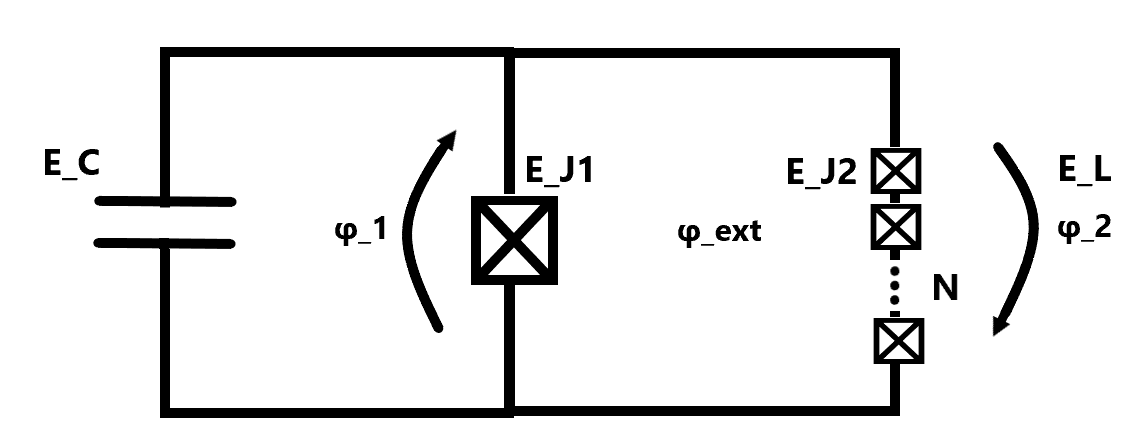
\includegraphics[width = 13cm]{Images/Fluxonium.png}
        \caption[Circuit diagram of a Fluxonium qubit]{\textbf{Circuit diagram of a Fluxonium qubit:} Schematic drawing of a Fluxonium qubit. The capacitor have energy $E_C$ and is connected to a Josephson junction with energy $E_{J_{1}}$ and an array of N Josephson junctions each with energy $E_{J_{2}}$. The array of Josephson junctions can be approximated as an inductor with energy $E_L$. There is a closed loop in the circuit to the right meaning we have a flux $\varphi_{ext} = \varphi_1 + \varphi_2$.}
        \label{fig:Fluxonium}
    \end{figure}
    %     It is 2 energy levels of the electrons (described collectively by a coherent macroscopic wave function) which we use as the qubit. 
    %     \\
    %     The collective wave function (and what state (energy) ) it is in, can be manipulated using a magnetic fields or gate voltages to change the superconducting phase or the number of electrons in the system. 
    %     \\
    %     We write the lagrangian in phase space
    %     - The hamiltonian
    % 			§ The approximation that we say that it is an inductor  - what the different terms are 
    %     - what the qubit is (the 2 level systems)
    %     - How do we experimentally (theoretically) simulate the Gates? 
    %     - How do we experimentally (theoretically measure?
    %     - Decoherence time for fluxonium 
    %     - Common noise in fluxonium? common problems 
    % Why is Fluxonium so much better than other qubits? 
    In fig. \ref{fig:Fluxonium} is a schematic of the Fluxonium circuit setup. It consists of a capacitor coupled in parallel to a Josephson junction and an array of Josephson junctions. The capacitor have a charging energy $E_C$ from the capacitor plates. The first Josephson junction (box with cross) have energy $E_{J_{1}}$ and the N Josephson junctions each give an energy-contribution of $E_{J_{2}}$. The contributions depend on the ratio,  $\gamma = E_{J2}/E_{J2}$, between the Josephson junction in the middle and the array of Josephson junctions on the right. Following the quasi-1D approximation, we get the following Hamiltonian \cite{Krantz2019}.
    \begin{equation}
        H \approx 4 E_C n^2-E_{J_{1}} \cos (\phi_1)- N \gamma E_{J_{2}} \cos (\frac{\phi_2}{N})
    \end{equation}
    Where the charging energy is $E_C = \frac{e^2}{2C}$ and C the capacitance of the capacitor. The Josephson energy is  $E_{J_{1(2)}} = \frac{I_{c1(2)}}{\phi_0}$ where $\phi_0 = \frac{\Phi_0}{2\pi}$ for the energy of the left(right) Josephson junction(s). Since we have a closed path = loop, we have an external flux given by: 
    \begin{equation}
        \phi_{ext} = \phi_1 + \phi_2 	\Leftrightarrow \phi_1 = \phi_{ext} -\phi_2
    \end{equation}
    We can approximate the array of Josephson junctions to have the total inductive energy $E_L = \frac{\gamma}{N} E_{J_{1}}$. Assuming N is large, we expand the 3rd term to a second order expansion. The flux Hamiltonian then becomes: 
    \begin{equation}\label{eq:hamiltonian_fluxonium}
        H = 4E_Cn^2- E_{J_{1}}cos(\phi_2 - \phi_e) + \frac{1}{2}E_L \phi_{2}^{2}
    \end{equation}
    By changing the ratio between $\varphi_{ext}, E_C, E_J$, and $E_J$ we can modify the energy spectrum. We want to find the some conditions for the ratio between the parameters such that the two lowest energy levels, $E_1$ and $E_2$, are well defined and close in energy, but with a large energy to the next energies. Therefore, we want a large anharmonicity between $\hbar \omega_{10}$ and $\hbar \omega_{21}$. We will explore the effects of varying parameters through a numerical simulation in Python, allowing us to systematically alter each parameter and observe its impact.

% \section{Gates - qubit - light coupling and qubit-qubit coupling described by cQED}
%     Circuit Quantum Electrodynamics(\acrshort{cqed}) is a theory describing the interaction between atoms or electrons and electromagnetic fields in quantum circuits (like superconducting circuits) \cite{Girvin2014}. This theory is useful because one uses light (microwave pulses) in order to control and manipulate the superconducting qubits (create superposition, entanglement etc.). we cannot ignore the interaction of light with our circuit anymore. The way of describing light    eg. by using  \acrshort{cqed} inspired from cavity \acrshort{qed} in quantum optics. 
%     \begin{itemize}
%         \item Draw your new circuit as a capacitative coupling between an ac(dc) light source and your transmon
%         \item write down you lagrangian
%         \item write down you hamiltonian
%         \item quantize it
%         \item transform it to the Fock space -> many body problem where you write it in terms of the creation and annihilation operator. 
%         \item dipole dipole approximation 
%         \item now you get a new Hamiltonian which have an interacting term describing the matter-light interaction. This look like the one we also see in rabi oscillations?? quantum optics "circuit QED"??
%     \end{itemize}
%     % How do we theoretically (maybe also computational control the Fluxonium qubits? we use Gates? but how? 
%     % \\
%     % You need a universal gate set - so you can get anywhere on the Bloch sphere. 
%     % \\
%     % Theoretical control - modify the energies (the voltage??)
%     % \\
%     % And experimental? Ground to excited states are controlled by microwave pulses
%     % \\
%     % Single Qubit Gates
%     % \\
%     % 2 Qubit gates
%     % picture of how you in theory experimentally couple 2 fluxonium qubits in order to be able to perform 2 qubit operations(gates) on them. 
%     % What their hamiltonian becomes (and in the computational part, you can compute  what their energy levels will become. and you can also then discuss how the $E_J$ compared to the $E_C$ etc. will become - just like for 

% \section{Decoherence time of qubits}  
    
% \section{Noise}
    
% \section{Readout}
%     Jaynes-Cummings hamilton is used in readout
    
    
\section{Noise and Decoherence time of qubits} 
% Decoherence time and noise:
% 	- What is coherence? Quantum coherence of a qubit is the property that allows superposition?? 
% 	- What is decoherence time? Decoherence time is the time it take for a quantum system to get entangled with the environment          which makes the system lose its coherence (quantum properties)
%   - What affect the decoherence time? How long time a qubit can maintain coherence is due to how it is build: 
%           - Material wise: 
%           - environmental wise: 
%   - what are the

% Dephasing should be high (how long it takes before the phase information is lost)
% Dephasing rate should be low (how fast it loses its phase information). 
% Coherence time should be long 
% Decoherence time should also be long


%  It is known that the Gamma_1 approximately increases with the external magnetic field for flux qubit. 
% Further they found out that \cite ( A scalable superconducting quantum simulator with long-range connectivity based on a photonic-bandgap metamaterial). 



% The coherence times of the qubits, which we expect to be limited by flux noise from on-chip sources [33], can be improved by reducing the loop size of the flux qubits and coupler, coupling the circuit elements galvanically rather than by a  mutual  inductance.   We  highlight  that  the  coupling scheme  is  compatible  with  other  qubit  modalities  such as  the  Transmon  [34]  or  fluxonium  qubit \cite(Demonstration of tunable three-body interactions between superconducting qubits) 



    We want to manipulate our qubits. However, there are some limitations of how long time the qubit can keep quantum coherence, that is be in a superposition. This is due to interaction(entanglement) with the environment. The interaction can be through thermal fluctuations,  electromagnetic radiation, or external noise. The time in which it is possible to manipulate the qubit, is called the coherence time. There are three commonly measures for the decoherence time:
    
    \paragraph{$T_1$} Is the energy relaxation time (or depolarization time). Due to the fact that there are an energy difference between the two states ($|0\rangle$ and $|1\rangle$) the qubit will at some point fall down to the lowest lying state. The time it takes is $T_1$. It is associated with the relaxation rate $1/\Gamma_1 = T_1$
    
    \paragraph{$T_{\phi}$} Is the pure dephasing time.  due to fluctuations, there will be a slight change of phase during an experiment. this is called the dephasing. The pure dephasing rate is: $1/\Gamma_{\phi} = T_\phi$

    % \paragraph{$T^{*}_{\phi}$} Is the inhomogeneous broadening time. Sometimes there will be some kind of drifting.The drifting rate is given by: $1/\Gamma^{*}_{\phi} = T^{*}_\phi$

    \paragraph{$T_2$} Is the total decoherence time and is given by the sum of the other decoherence times: 
        \begin{equation}\label{eq:total_decoherence}
            \frac{1}{T_2} = \frac{1}{2T_1} + \frac{1}{T_{\phi}} 
        \end{equation}

    $T_1$ can be directly measured, but it is not possible to experimentally measure $T_{\phi}$. Therefore you use eq. \ref{eq:total_decoherence} to find $T_2$. There are 2 approaches to find this. Either by using ramsey or echo. 
        
    \paragraph{$T_2, ramsey$}
        
    \paragraph{$T_2,echo$}
        Its the same as $T_2$, but it take into account the external noise by using 


% \section{Readout}

% \section{Gates}
%     In order to perform all the operations we want, You need a universal gate set,  so you can get anywhere on the Bloch sphere. 
%     \\
%     Theoretical control, modify the energies (the voltage??)
%     \\
%     And experimental? Ground to excited states are controlled by microwave pulses
    
%     \subsection{single qubit gates}
%         Single Qubit Gates
        
%     \subsection{2 qubit gates}
%         picture of how you in theory experimentally couple 2 fluxonium qubits in order to be able to perform 2 qubit operations (gates) on them. 
%         What their hamiltonian becomes and in the computational part, you can compute  what their energy levels will become. And you can also then discuss how the $E_J$ compared to the $E_C$ etc. Will become just like for. 